\documentclass[a4paper,11pt]{article}
\usepackage[utf8]{inputenc}
\usepackage[T1]{fontenc}
\usepackage[french]{babel}
\usepackage{amsmath, amssymb}
\usepackage{graphicx}
\usepackage{listings}
\usepackage[top=2cm, bottom=2cm, left=2cm, right=2cm]{geometry}
%\usepackage[vlined,lined,linesnumbered,boxed,french]{algorithm2e}
\usepackage{tikz}
\usetikzlibrary{arrows,automata,shapes}

\lstdefinestyle{customc}{
  belowcaptionskip=1\baselineskip,
  breaklines=true,
  frame=L,
  xleftmargin=\parindent,
  language=C,
  showstringspaces=false,
  basicstyle=\footnotesize\ttfamily,
  keywordstyle=\bfseries\color{green!40!black},
  commentstyle=\itshape\color{purple!40!black},
  identifierstyle=\color{blue},
  stringstyle=\color{orange},
}
\lstset{escapechar=@,style=customc}

\newcommand{\inlinecode}[2]{\colorbox{white}{\lstinline[language=#1]$#2$}}

\author{Emeric Duchemin, Laurent Genty, Julien Miens, Tanguy Pemeja}
\title{Rapport de Projet - BitBoards}

\begin{document}

\thispagestyle{empty}
~
\vfill
\begin{center}
    
\includegraphics[width=0.3\textwidth]{logo}\\[0.5cm]

    \LARGE Filière informatique\\
    \LARGE \bsc{Enseirb-Matmeca}\\[1.5cm]
    {\Large \bfseries \bsc{--- Projet Semestre 6 ---}}\\[0.5cm]
    \scshape
	\vspace*{\baselineskip}
	\rule{\textwidth}{1.6pt}\vspace*{-\baselineskip}\vspace*{2pt}
	\rule{\textwidth}{0.4pt}
	\vspace{0.\baselineskip}

    {\LARGE \textbf{Bitboard - Jeu de Gomoku}}
	\vspace{0.65\baselineskip}

	\rule{\textwidth}{0.4pt}\vspace*{-\baselineskip}\vspace{3.2pt}
	\rule{\textwidth}{1.6pt}
    {\Large Emeric \bsc{Duchemin} \quad Laurent \bsc{Genty} \\\quad Julien \bsc{Miens} \quad Tanguy \bsc{Pemeja}}\\[0.5cm]
    {\large Encadré par Frédéric \bsc{Herbreteau}}\\
    \vfill
    {\large Mars -- Mai 2019}
    \vfill
    ~
\end{center}
\newpage

\tableofcontents
\listoffigures

\newpage


\section*{Introduction}

% étape 1 : le jeu
Le Gomoku est un jeu d'origine asiatique consistant à aligner 5 pions sur un plateau de Go. Deux joueurs s'affrontent, l'un ayant les pions noirs, l'autre les blancs.
% étape 2 : le server
Afin de pouvoir gérer le jeu, un serveur se chargera de faire intéragir les joueurs en leur demandant les coups qu'ils veulent et en les communiquant aux autres. Ensuite, il va stocker ces mouvements pour remplir son plateau de jeu, vérifier leur validité et potentiellement terminer la partie si la situation se trouve dans un cas gagnant.
% étape 3 : le bitboard
Le plateau de jeu quant à lui, est une grille carrée contenant tous les coups posés par les joueurs. Ce plateau peut être réalisé de différentes manières plus ou moins efficaces. Il peut être vu comme une matrice, un tableau ou même un nombre dont les bits correspondent à une case du plateau.
% étape 4 : le joueur
Le joueur utilise une stratégie de type minimax, très utile dans le contexte de ce type de jeu à deux joueurs. Le principe est de tenter de prédire le futur en se mettant à la place de l'adversaire afin d'en déduire le meilleur coup possible. L'heuristique, permettant de n'explorer que les coups les plus prometteurs, donne une valeur à chaque coup possible selon les lignes qui seraient formées (et qui se croiseraient) si on jouait le coup. Le parcours de l'arbre est optimisé en utilisant l'élagage Alpha-Bêta, permettant de ne pas considérer des branches pour lesquelles on connaît déjà une meilleure solution, et le calcul parallèle des noeuds fils de la racine.
% étape 5 : les résultats
Les fonctions d'heuristique implémentées par le minimax doivent être testées afin de valider ou invalider l'efficacité de celles-ci. Les tests peuvent être réalisés pour évaluer les openings dans le cadre de joueurs parfaits.

%%%%%%%%%%%%%%%%%%%%%%%%%%%%%%%%%%

\section{Server}
\label{sct:server}

Afin de pouvoir échanger les informations concernant le déroulement de la partie et les joueurs, l'implémentation d'un serveur est primordiale. Ce serveur aura pour rôle de :

\begin{itemize}
    \item organiser la partie : donner les conditions de jeu initiales
    \item faire jouer chaque joueur : leur demander les coups qu'ils veulent jouer
    \item vérifier la validité des coups
    \item envoyer les $n$ derniers coups à chaque joueur
\end{itemize}

Lorsque l'on parle de conditions initiales, cela signifie : la taille du plateau, le nombre de joueurs, si la partie s'effectue en mode normale ou bien en mode \textit{swap}. En effet, dans le jeu officiel du Gomoku, il est possible de démarrer une partie dans un mode \textit{swap} permettant de proposer des openings aux parties.

Le mode standard consiste à faire démarrer les deux joueurs sur un plateau vide avec comme joueur aux pions noirs le joueur 1. Lorsque l'option est activée, elle permet au premier joueur de proposer une suite de 3 coups valides sur le plateau sous la forme de (NOIR,BLANC,NOIR). Le deuxième joueur peut donc accepter (ou refuser) et commencer la partie en jouant les blancs. S'il refuse il joue les noirs et l'autre joueur devenu blanc peut commencer la partie.

%%%%%%

\subsection{Implémentation de types abstraits de données relatifs au serveur}
\label{subsct:tad_server}

 Les structures \inlinecode{C}{struct move_t} et \inlinecode{C}{struct col_move_t} permet déjà de représenter les mouvements sur un plateau. Il s'agit seulement de structures ayant des positions $i$ et $j$ (et une couleur pour \inlinecode{C}{struct col_move_t}). Mais où les stocker ?
 Afin de pouvoir envoyer les informations aux joueurs, nous avons décidé d'implémenter différents types abstraits de données qui permettent de représenter la suite des mouvements effectués sur le plateau.

La structure \inlinecode{C}{struct moves} permet de modéliser ces mouvements par le serveur :

\begin{lstlisting}
    struct moves {
        struct col_move_t* t;
        size_t size;
    };
\end{lstlisting}
\label{lst:struct_moves}

Cette structure va permettre de stocker les $n$ derniers mouvements du plateau effectués par les joueurs. Contrairement à la gestion des mouvements des joueurs qui stockent tous les mouvements, nous avons fait le choix de prendre un \inlinecode{C}{struct col_move_t* t} de \textbf{taille $4$}. En effet, selon nous, il était beaucoup plus pertinent de construire un type abstrait de données se limitant seulement aux 4 derniers coups (même si l'on remplit généralement deux cases, le cas de l'opening est lui traité). Le serveur, à chaque coup, vérifiera la validité des coups, et seulement s'ils sont valides va les placer dans son plateau. Il n'est donc pas nécessaire d'avoir en mémoire tous les coups.

Ces coups seront donc donnés aux joueurs avec notamment la fonction \inlinecode{C}{moves__last_n(moves)}, afin qu'ils puissent remplir leur plateau interne.

Comme nous l'avons dit, le remplissage varie donc de $1$ à $4$. En effet, si l'option permettant de jouer les openings est utilisée, alors le tableau sera remplie au $\frac{3}{4}$. Si le joueur adverse accepte alors l'opening, le tableau renvoyé remplie $4$ après le vrai premier coup de la partie. Et une fois que ce premier coup est joué, alors le tableau contient $2$ éléments jusqu'à la fin de la partie.

\bigbreak

Dans la mesure où le serveur doit pouvoir gérer les différents joueurs d'une partie de Gomoku, nous avons aussi décidé d'implémenter un autre type abstrait de données concernant les joueurs. Des \textit{joueurs} : \inlinecode{C}{struct player_t} contenus un tableau de joueur : \inlinecode{C}{struct player_t players[NB_PLAYERS]}.

Cette structure est donc composée de pointeurs de fonctions vers les différentes fonctions qui nous ont été imposées dans la consigne. \`A savoir :

\begin{lstlisting}
    struct player_t {
        char const* (*get_player_name)(void);
        struct col_move_t* (*propose_opening)(size_t);
        int (*accept_opening)(size_t,const struct col_move_t*);
        void (*initialize)(size_t,enum color_t);
        struct move_t (*play)(const struct col_move_t*,size_t);
        void (*finalize)(void);
        void* handle;
    };
\end{lstlisting}
\label{lst:struct_player_t}

Ces fonctions seront liées avec celles du joueur notamment grâce à la bibliothèque \verb+dlfcn.h+ nous permettant de trouver l'adresse des symboles de fonctions données par une librairie dynamique (à savoir celles des joueurs compilés en \verb+.so+). Cette librairie sera notamment stockée dans le \verb+void* handle+ pour pouvoir ensuite la fermer.

Le choix d'avoir créer cette structure a été effectué dans l'optique d'avoir un code adaptable et surtout évolutif. Si l'on souhaite faire évoluer le jeu avec $3$ joueurs ou plus, alors cette structure pourrait être facilement adaptée. De cette manière, le serveur n'a pas à se soucier du nombre de joueurs ou bien de leur initialisation, c'est le type abstrait de données \verb+players+ qui s'en chargera.
De plus, le fait de mettre un type abstrait de données au dessus des "vrais" joueurs, nous permet de rendre n'importe quel joueur générique. Si l'on prend un joueur d'un autre groupe, notre serveur récupérera seulement les fonctions dont il se sert (et qui sont donc dans la structure) et traitera désormais le joueur non plus comme un \inlinecode{C}{struct playerXXX} quelconque d'une autre équipe, mais bien comme un \inlinecode{C}{struct player_t}.

%%%%%%

\subsection{Initialisation et déroulement du jeu}
\label{subsct:init_game}

Afin de lancer le jeu, il est nécessaire de poser des conditions de base qui \textbf{seront utilisées}.
Pour ce faire il faut lancer le serveur en donnant les informations relatives à la partie :
\begin{verbatim}
    ./server player4.4.so player4.3.so -n 10 -o
\end{verbatim}

En début d'exécution le serveur va donc initialiser tout le jeu avec : le plateau \textit{bitboard}, les joueurs \inlinecode{C}{player_t}, la liste des mouvements initiaux (vide au départ)
La taille du plateau peut être indiquée : \verb+-n 10+. Cette information sera  utile dans la mesure où l'ensemble des algorithmes et structures interagissant avec le serveur auront besoin de la taille de la grille afin de pouvoir eux-mêmes se créer leur plateau.

Comme expliqué plus tôt dans cette Section, grâce à l'option \verb+-o+ durant l'exécution du programme, il est possible d'indiquer au serveur que nous souhaitons effectuer une partie avec un opening. Si tel est le cas, alors le premier joueur proposera un opening parmi les siens et le serveur l'ajoutera dans le tableau des mouvements. Après l'accord ou le refus de l'autre joueur, le jeu pourra commencer.
A chaque tour, le serveur envoie les $2$ derniers coups à un joueur, qui va lui renvoyer son coup calculé. Si le coup est valide alors il l'ajoute dans sa liste des $n$ derniers coups, il supprime le coup joué le plus ancien et ajoute le nouveau. Cependant si le plateau est rempli ou bien qu'il y a une situation gagnante pour l'un des joueurs, alors la partie se termine. Si non, la partie continue.

%%%%%%%%%%%%%%%%%%%%%%%%%%%%%%%%%%

\section{BitBoard}
\label{sct:bitboard}

Nous décrivons ici différentes approches afin de réaliser le plateau de jeu ainsi que diverses fonctions utilisant ce dernier. Dans un premier temps, nous différencierons $2$ possibilités d'implémentations, l'une sous la forme d'un tableau contenant toutes les cases du plateau, l'autre sous la forme d'un entier dont les bits forment les différentes cases.

%%%%%%
\subsection{Plateau de jeu}
\label{subsct:plateau}

Le plateau de jeu est constitué d'une grille carrée. Naturellement, nous avons envisagé de partir sur une matrice ou un tableau de tableau d'entier afin de réaliser le plateau. Mais cette idée a rapidement été écartée du fait d'un surplus d'espace utilisé lors des rappels répétés à malloc. L'idée a été alors de réserver un espace mémoire sous forme de tableau d'entier suffisamment grand pour représenter toutes les cases.
\begin{figure}[h]
    \centering
    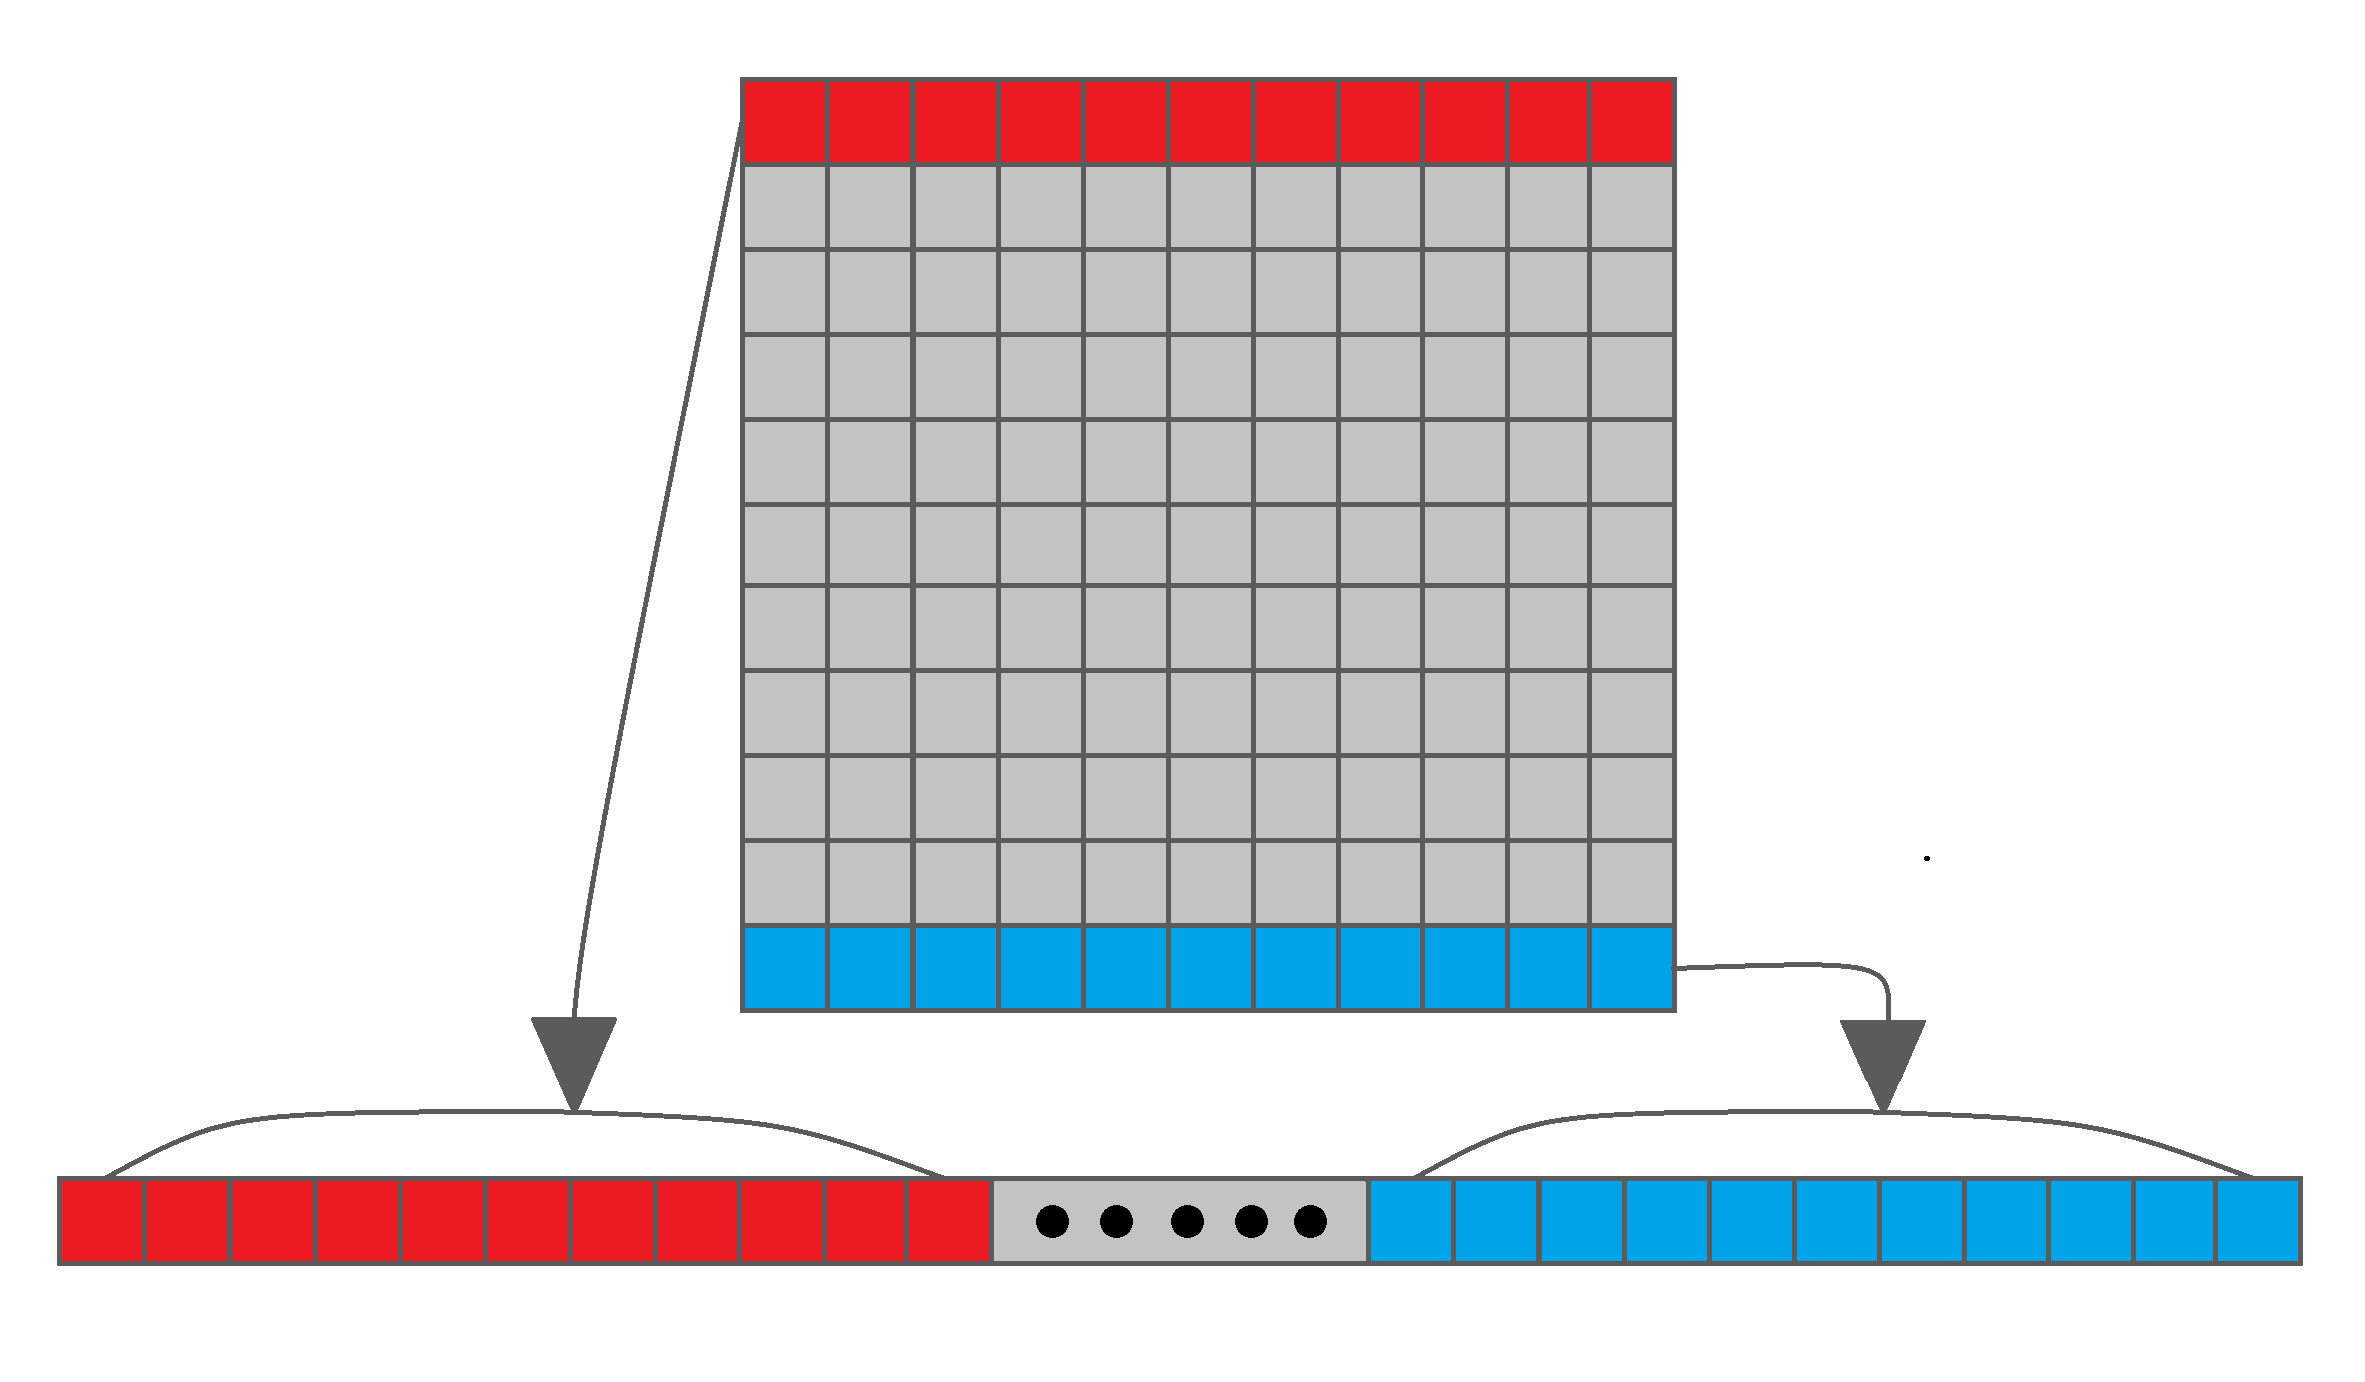
\includegraphics[scale=0.20]{Board_en_ligne.png}
    \caption{Représentation du plateau sous la forme d'un tableau}
    \label{fig:Board_ligne}
\end{figure}

\bigbreak

Cependant, ce choix n'est pas très pertinent. En effet, afin de pouvoir vérifier si le plateau est rempli ou bien que certains schémas sont obtenus, il faudrait comparer chacune des cases de la matrice, ce qui aurait compliqué le code, ou tout du moins, l'aurais alourdi.

Le choix effectué est donc celui de représenter ce tableau sous la forme d'entiers. Nous avons donc changer notre implémentation du plateau comme sur la Figure \ref{fig:Tabtobitboard}.

En effet, en considérant un entier de $128$ bits, il est possible de représenter un plateau d'une taille d'au plus $11\times11 = 121\,cases$.

\begin{figure}[h]
    \centering
    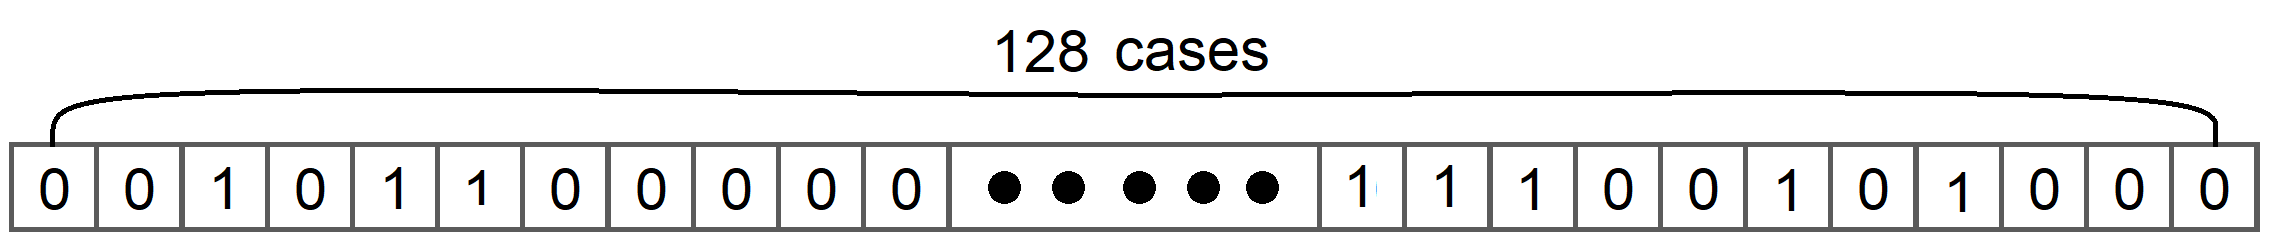
\includegraphics[scale=0.20]{Int_128.png}
    \caption{Représentation d'un entier de $128$ bits}
    \label{fig:Int_128}
\end{figure}

\bigbreak

Contrairement à un tableau d'entier qui peut avoir $3$ états différents dans notre cas, $-1$ lorsqu'il n'y a pas de pion et $0,1$ pour les pions des joueurs respectifs, un entier ne peut prendre que $2$ états distincts: $0$ ou $1$. Dès lors, il est nécessaire d'avoir $2$ entiers de $128$ bits afin de représenter le plateau. Chaque entier représente un joueur avec pour chaque bit, la valeur $1$ si le joueur a un pion dans cette case et $0$ sinon. Dans le type abstrait de données du plateau, il y a bien deux entiers non signés de $128$ bits chacun comme montré sur la Figure \ref{fig:Int_128} :

\begin{lstlisting}
    struct board{
      __uint128_t* b_w;
      __uint128_t* b_b;
      size_t capacity;
  };
\end{lstlisting}
\label{lst:struct_board}

Il est important de noter que notre séquence de bits ne contient aucun bit de séparation concernant les lignes.

\begin{figure}[h]
    \centering
    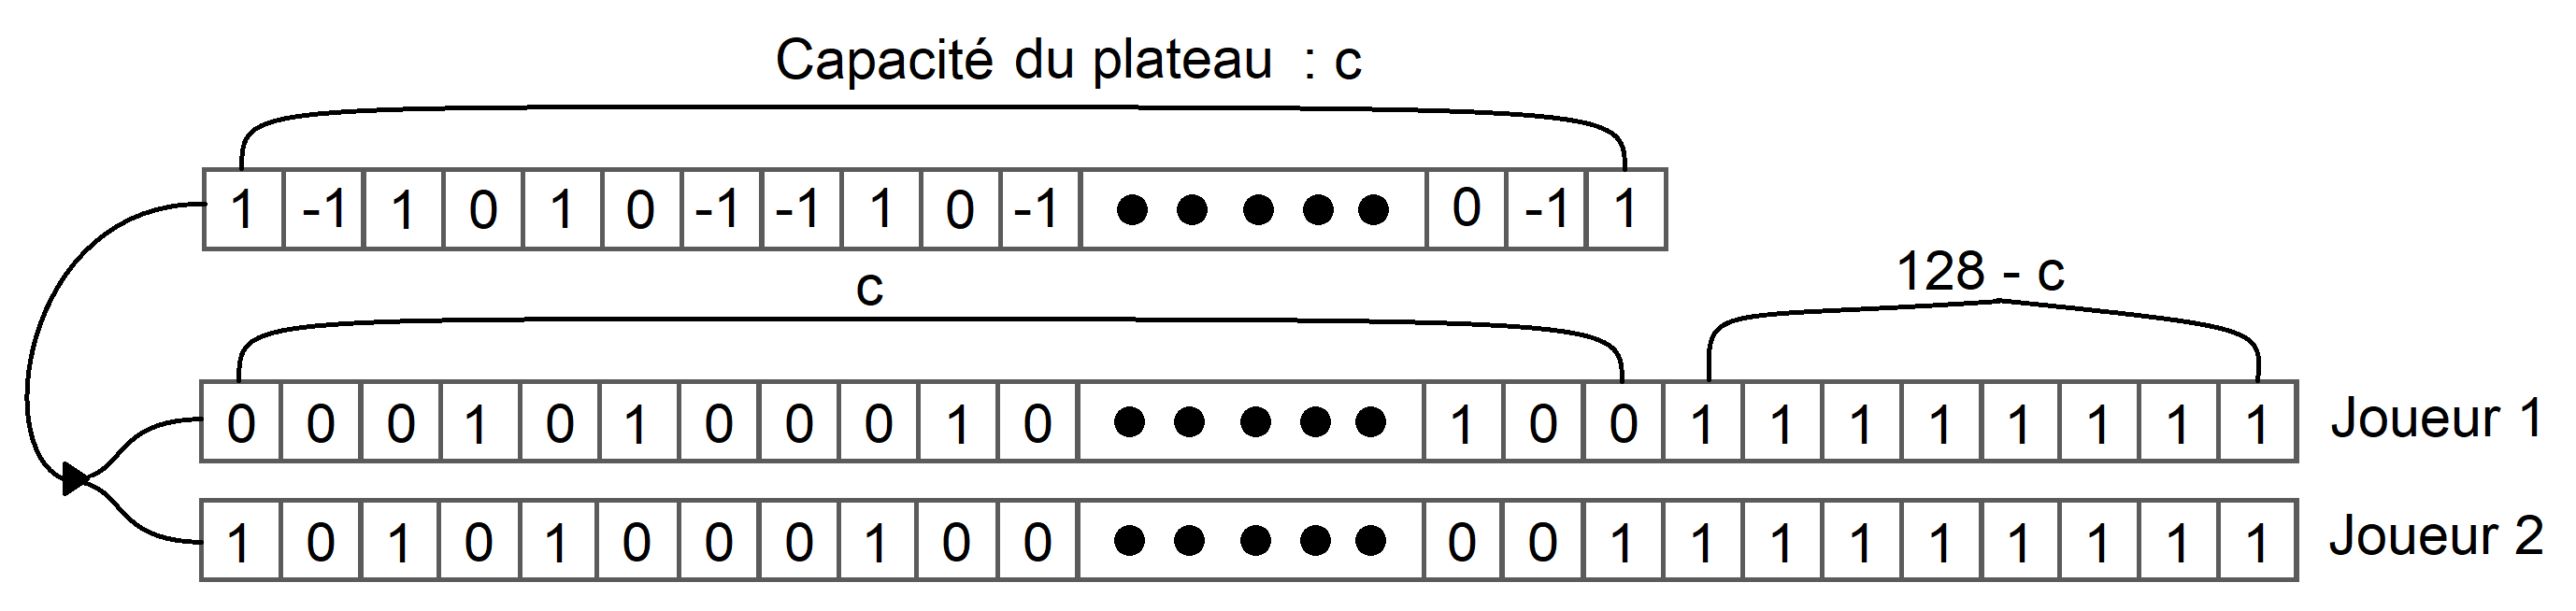
\includegraphics[scale=0.20]{Board_ligne_en_int.png}
    \caption{Passage d'un tableau d'entier en bitboard}
    \label{fig:Tabtobitboard}
\end{figure}

%%%%%%

\subsection{Fonctions basées sur le bitboard nécessaire à l'implémentation du jeu}
\label{subsct:fct_bitboard}

Suite à la création du \textit{bitboard}, nous avons implémenté des fonctions utilisant ce \textit{bitboard} et réalisant les fonctions suivantes, nécessaires à l'implémentation du jeu :

\begin{itemize}
    \item[$\bullet$]
    \inlinecode{C}{int board__position(size_t size,int i,int j)}
     \\ Cette fonction retourne la position dans le tableau pour une case situé à la i-ème ligne et j-ème colonne grâce à la formule :
    \begin{equation}
    \label{eq:position}
    position = i\times n_{plateau}+j
    \end{equation}
    \\
    \item[$\bullet$]
    \inlinecode{C}{__uint128_t board__select_bit(__uint128_t* b, int pos)}
    \\ Pour un entier de 128 bits et une position, la fonction retourne la valeur du bit de l'entier à cette position. Pour cela, on décale les bits du nombre vers la gauche de \textit{position-1} bits. Et par le résultat du \verb+ET+ logique entre ce nombre décalé et l'entier $1$, il est possible de déterminer la valeur du bit de l'entier à la position comme sur la Figure \ref{fig:selectbit}
    \begin{figure}[h]
    \centering
    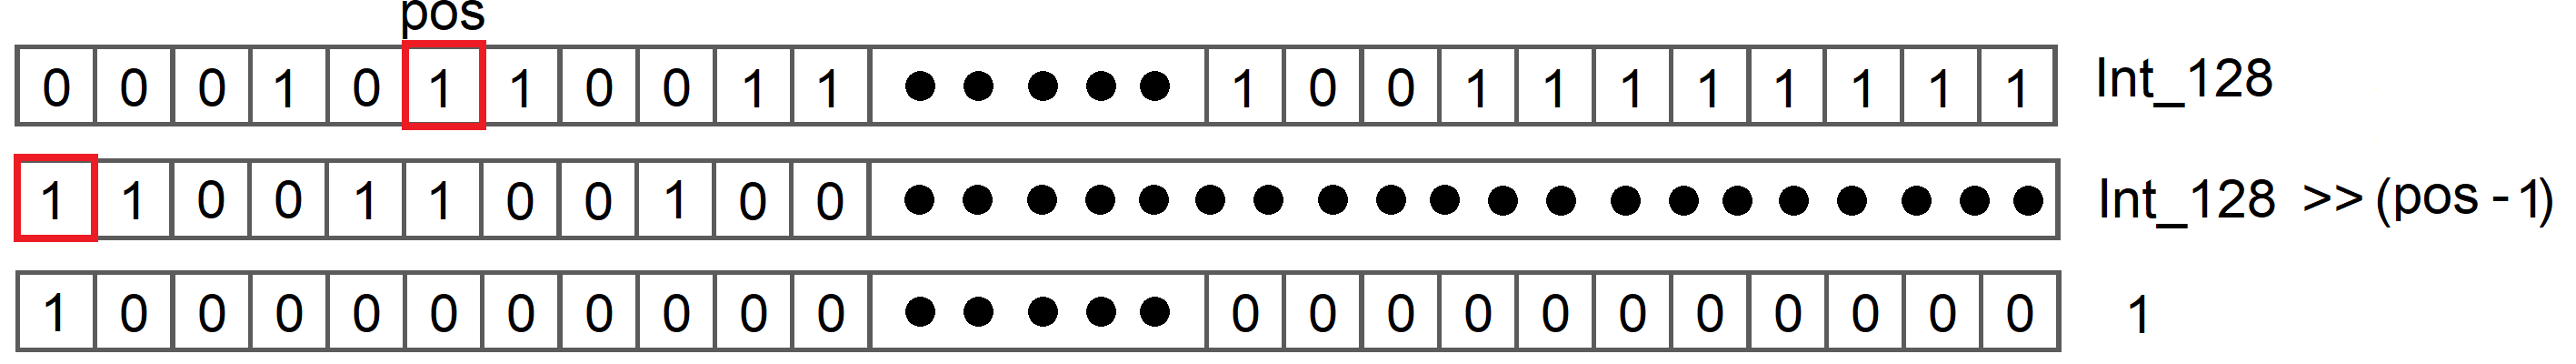
\includegraphics[scale=0.20]{board_select_bit.png}
    \caption{Détermination du bit à une position}
    \label{fig:selectbit}
    \end{figure}
    \item[$\bullet$]
    \inlinecode{C}{struct board * board__initialize(size_t size)}
    \\ Cette fonction réserve un espace mémoire suffisant à l’implémentation du plateau c'est-à-dire $2$ entiers représentant les $2$ joueurs. Cette fonction initialise les derniers bits des $2$ entiers non utilisés dans la réalisation du plateau à $1$ comme montré sur la Figure \ref{fig:boardinit}
    \begin{figure}[h]
    \centering
    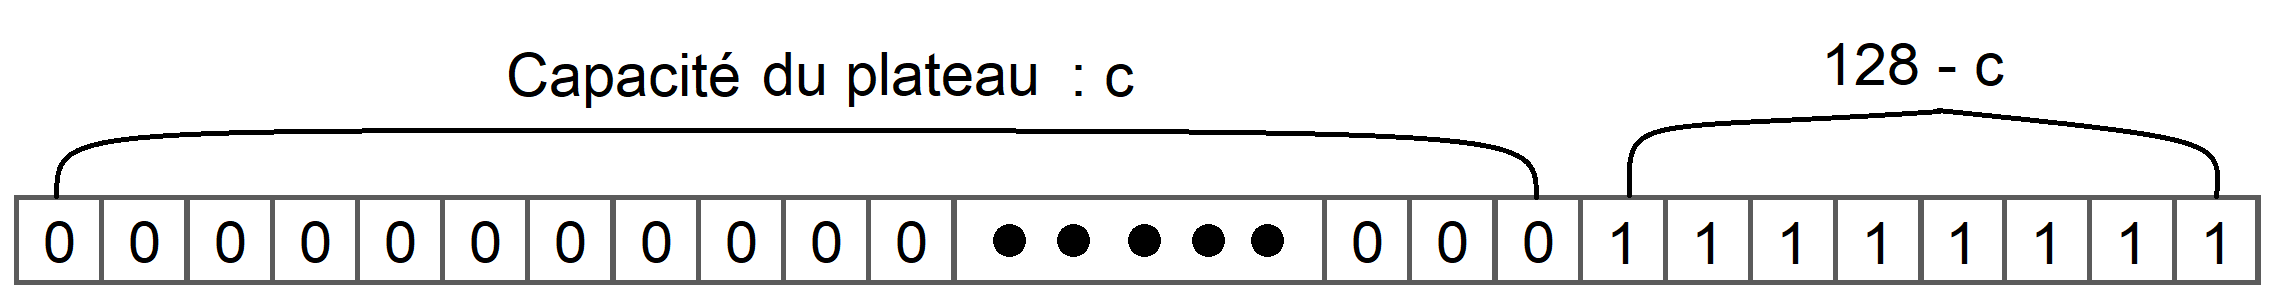
\includegraphics[scale=0.20]{Birboard_init.png}
    \caption{Initialisation du bitboard}
    \label{fig:boardinit}
    \end{figure}
    \\ Ce choix a un prix, il est lourd au départ de la partie cependant il permet d'optimiser le temps nécessaire afin de savoir si le plateau est rempli ou non.
    \\
    \item[$\bullet$]
    \inlinecode{C}{int board__is_full(struct board* board)}
    \\ Grâce à une telle initialisation, il est possible de déterminer si le plateau est rempli en temps constant grâce aux opérations binaires (ce que nous ne pouvions pas faire avec l'ancienne implémentation). Le \verb+ET+ logique entre les entiers représentant les 2 joueurs nous permet d'obtenir le plateau. Et pour savoir si celui-ci est plein il nous suffit alors de tester si le résultat de ce \verb+ET+ est égal au $-1$ qui représente l'entier dont tout les bits sont égaux à $1$ comme sur la Figure \ref{fig:boardfull}
    \begin{figure}[h]
    \centering
    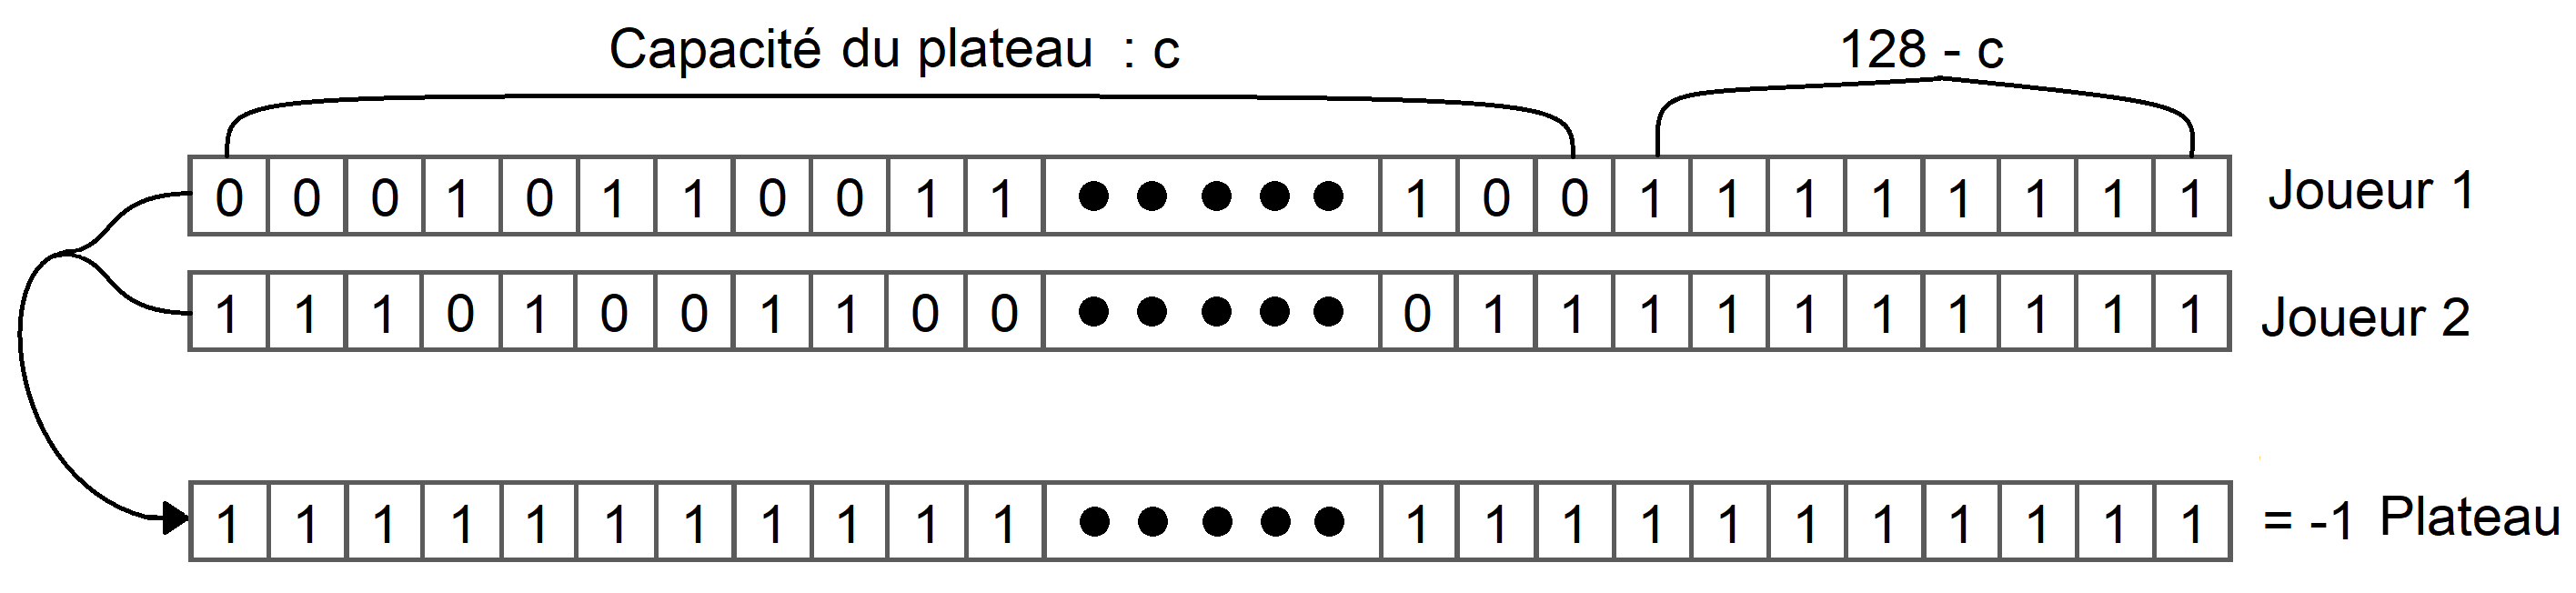
\includegraphics[scale=0.20]{board_full.png}
    \caption{Test pour savoir si le plateau est rempli complètement}
    \label{fig:boardfull}
    \end{figure}
    \\
    \item[$\bullet$]
    \inlinecode{C}{int board__is_valid_move(struct board* board, struct move_t move)}
    \\ Pour déterminer si un coup $(i,j)$ est valide il suffit de déterminer sa position grâce à la formule \ref{eq:position}.
    Si cette position n'appartient pas au plateau on retourne faux sinon en retournant la négation du bit du plateau pour cette position, nous obtenons le booléen déterminant si le coup est valide ou non.
    \\
    \item[$\bullet$]
    \inlinecode{C}{void board__add_move(struct board *b, struct move_t move, enum color_t i)}
    \\
    En connaissant la couleur du joueur qui joue le coup, il est facile d'ajouter un coup valide dans le plateau. En effet, en déterminant la position du coup comme précédemment, nous obtenons le nouvel entier représentant les coups du joueur en faisant un \verb+OU+ logique entre l'entier du joueur et l'entier 1 décalé vers la droite de $pos$ bits comme montré sur la Figure \ref{fig:addmove}
    \\
    \begin{figure}[h]
    \centering
    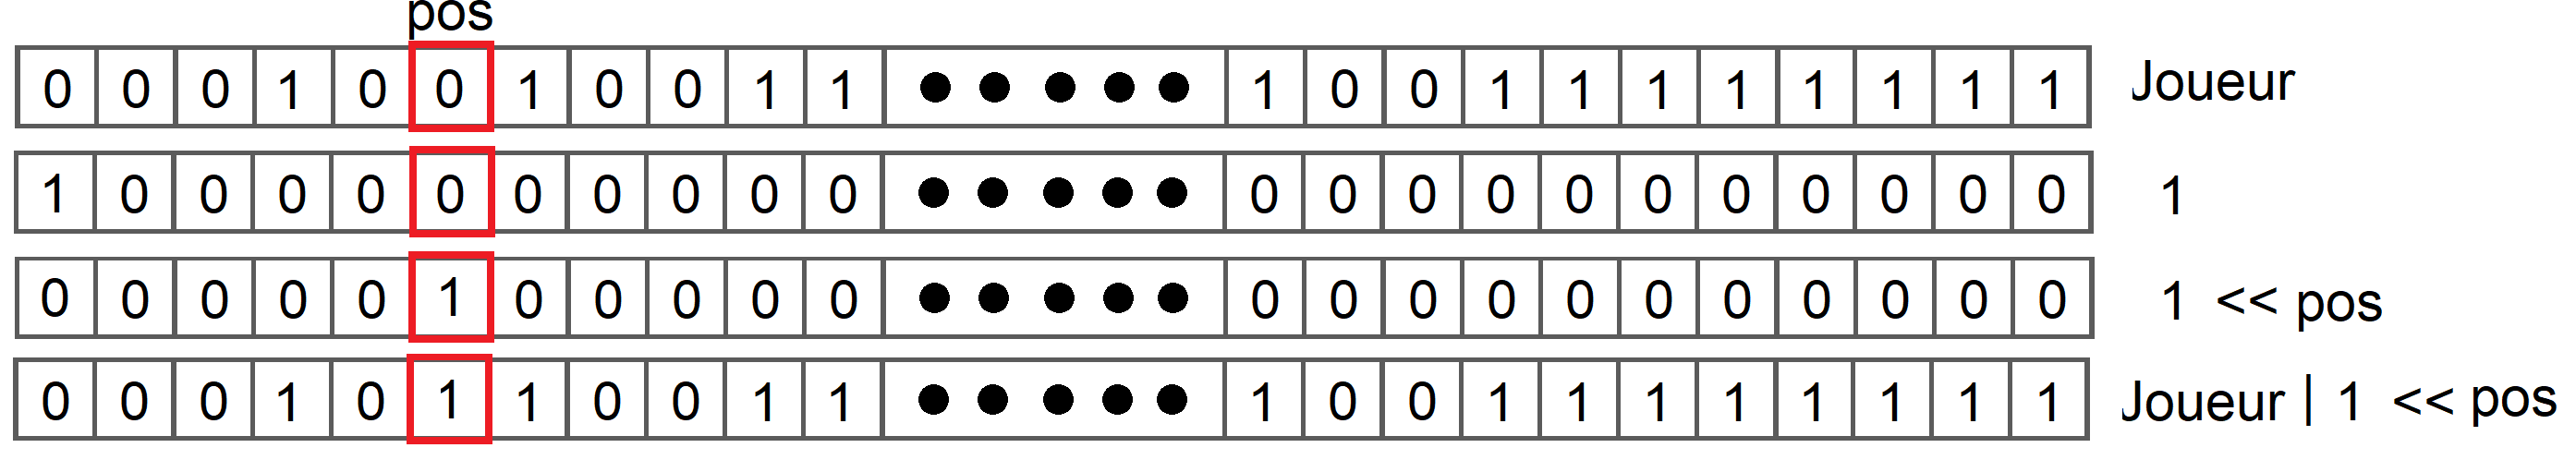
\includegraphics[scale=0.20]{board_add_move.png}
    \caption{Ajout d'un coup aux coups d'un joueur}
    \label{fig:addmove}
    \end{figure}
    \\
    \item[$\bullet$]
    \inlinecode{C}{int board__won(struct board* board, struct move_t move)}
    \\
    Cette fonction permet de déterminer si le dernier coup joué à permis au joueur de gagner. Pour cela nous devons identifier et analyser toutes les lignes de 5 pions incluant le coup et pouvant entraîner une victoire comme sur la Figure \ref{fig:checkmove}
    \begin{figure}[h]
    \centering
    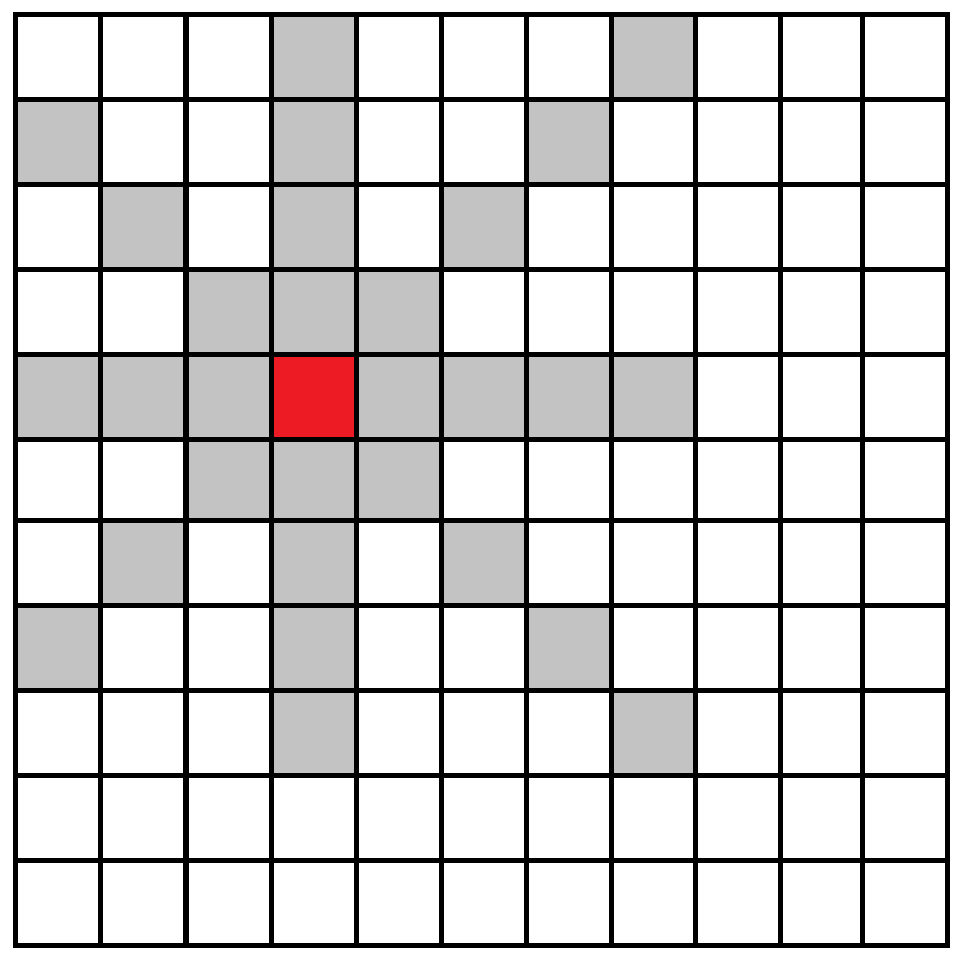
\includegraphics[scale=0.20]{board_check.png}
    \caption{Détermination de toutes les lignes contenant le coup}
    \label{fig:checkmove}
    \end{figure}
    \\La logique étant identique pour chaque direction, nous allons traiter ici que le cas horizontal.
    \\Dans notre implémentation, nous sommes parti du principe que l'étude de chaque ligne s'effectuait en comparant la valeur de 5 cases successives.
    \begin{figure}[h]
    \centering
    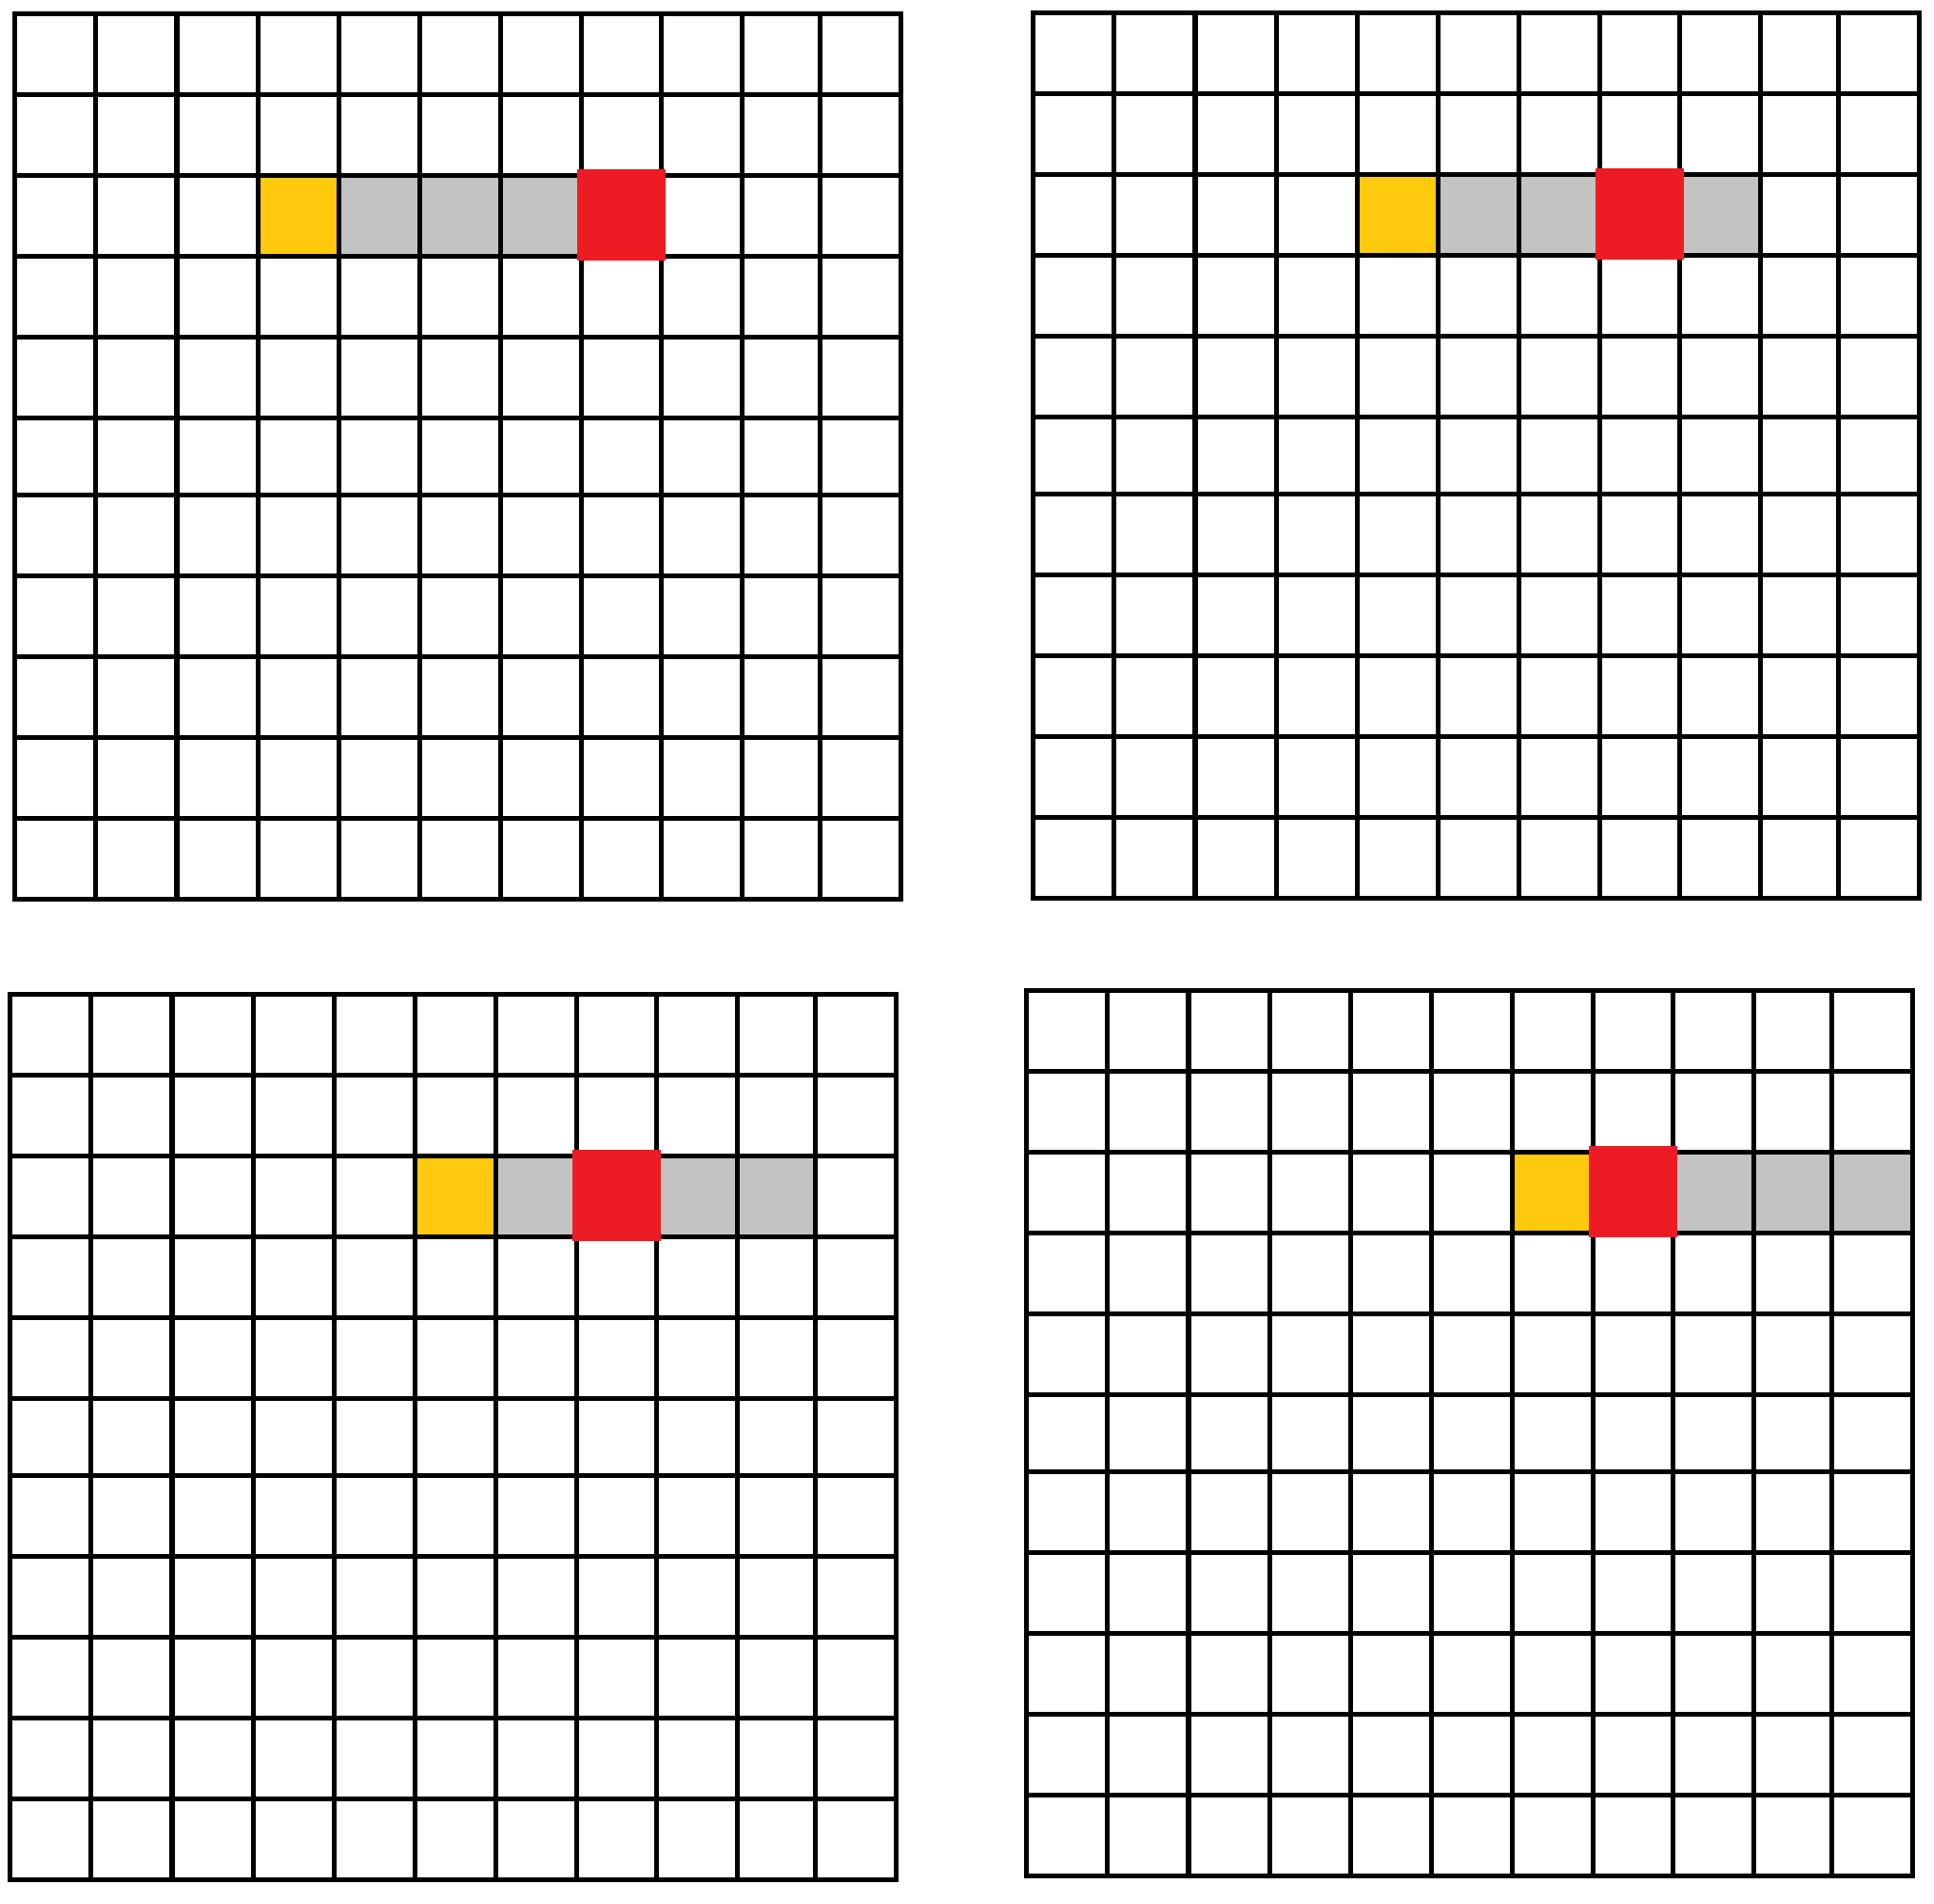
\includegraphics[scale=0.15]{horizontal.png}
    \caption{Différentes positions de départs de ligne de 5 contenant la case rouge}
    \label{fig:horizontal}
    \end{figure}
      Ainsi il faut déterminer l'ensemble des 5 cases contenant le coup et vérifier si ces cases sont identiques. Pour cela, nous utilisons un masque, où chaque bit de valeur 1 représente une case vérifiée. \\
      Pour cela, nous avons une fonction qui détermine la position initiale du masque, telle que la position soit la première position des 5 premières cases valides et consécutives contenant le dernier coup joué et ceux grâce à la formule suivante :
  \begin{equation}
  \label{pos_init}
    position\_initiale=
    \begin{cases}
      i\times n_{plateau}+(j-4), & \text{si}\ (j \geqslant 4) \\
      i\times n_{plateau}, & \text{sinon}
    \end{cases}
  \end{equation}
\\Après avoir déterminer cette position initiale, il est nécessaire de construire un masque afin de l'appliquer à l'entier représentant les coups du joueur. Nous créons ce masque par décalage de celui-ci et \verb+OU+ logique avec 1 comme décrit dans la figure \ref{fig:mask} ci-dessous.
    \begin{figure}[h]
    \hspace{3 cm}
    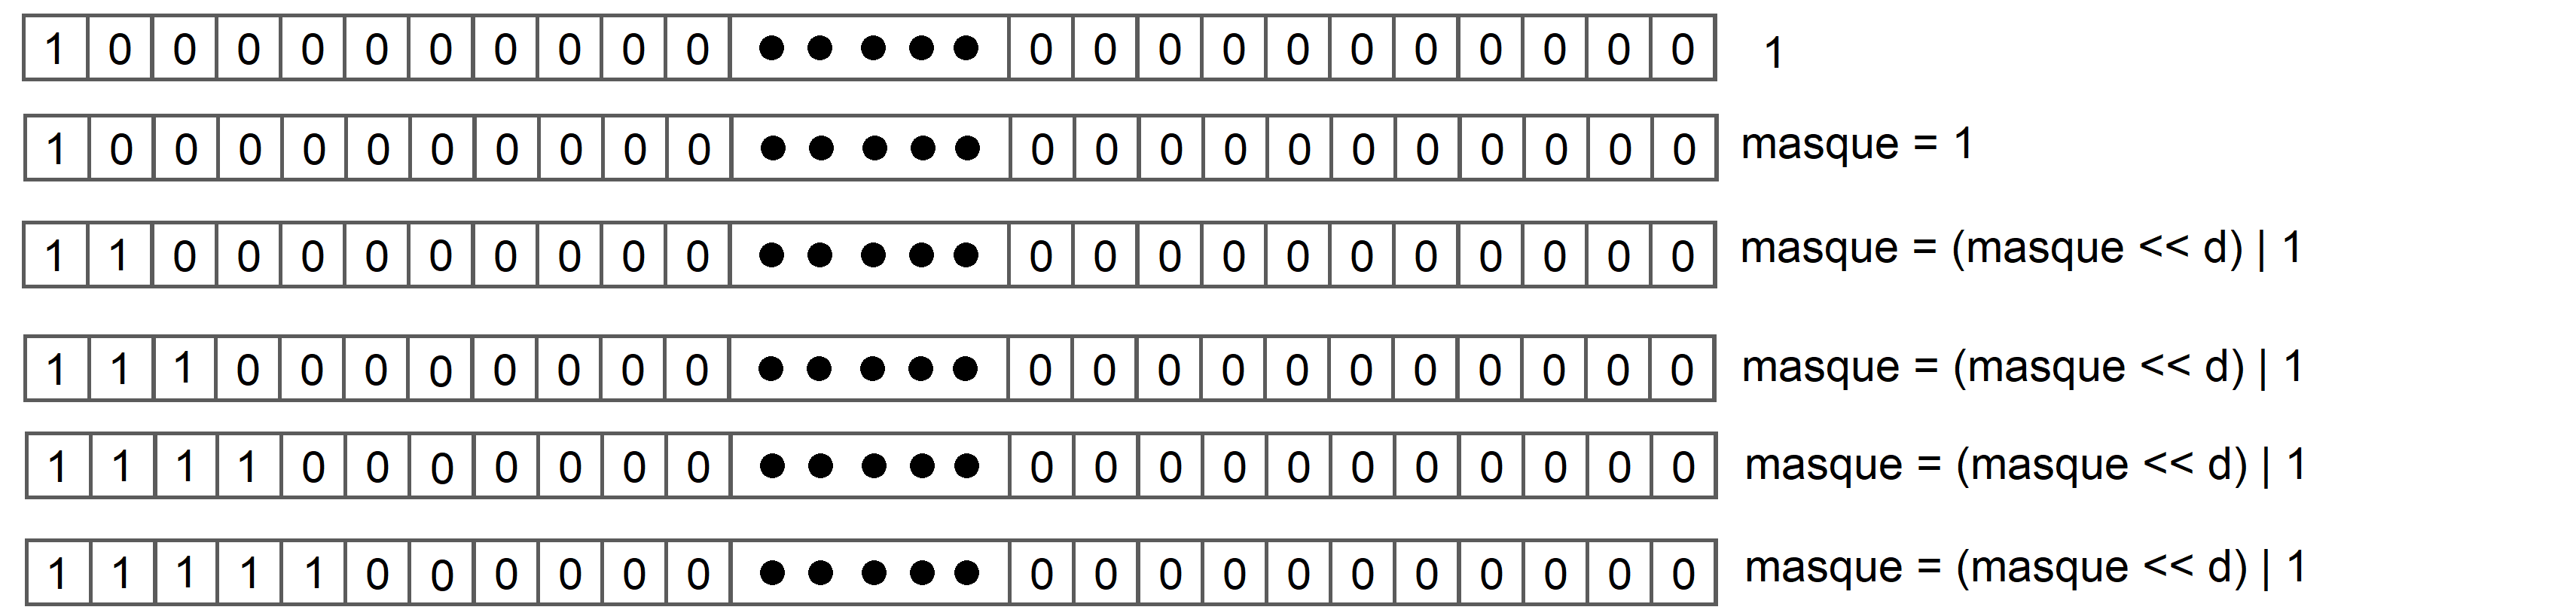
\includegraphics[scale=0.2]{creation_masque.png}
    \caption{Création d'un masque}
    \label{fig:mask}
    \end{figure}
    \\  Afin de générer nos masques suivant les différentes directions, nous modifions uniquement la valeur du décalage d.
    \begin{figure} [h]
\caption{\label{tab1} Tableau des décalages suivant les directions pour un plateau de taille $n\times n$}
\centering
\begin{tabular}{|c|c|}
    \hline
    Direction & valeur du décalage  \\
    \hline
    Horizontale & 1 \\
    Verticale & n \\
    Diagonale Nord-Ouest/Sud-Est & n+1 \\
    Diagonale Sud-Ouest/Nord-Est & n-1 \\
    \hline
\end{tabular}
\end{figure}
\\
Notons que le masque pour une ligne horizontale s'obtient plus rapidement en prenant directement le nombre 31 (11111 en binaire). Une fois obtenu ce masque nous le décalons vers la gauche de \textit{position\_initiale} bits afin que le premier 1 du masque correspond à la première case de la première ligne de 5 pions contenant le coup joué.
\\ On peut alors effectuer un \verb+ET+ logique entre le masque et l'entier du joueur afin d'obtenir le booléen représentant si la ligne est une ligne de 5 pions alignés. Si ce n'est pas le cas, nous décalons la masque de la même distance d vu précédemment. En faisant attention toutefois car dans l'exemple de la figure \ref{fig:horizontal}, nous pouvons remarquer qu'il n'y a que 4 possibilités telles que la case rouge appartienne à une ligne de 5 et ceux à cause de la limite du plateau. Ainsi avant de décaler notre masque nous devons vérifier que la dernière case de la nouvelle ligne reste valide.
    \\
    \item[$\bullet$]
    \inlinecode{C}{void board__free(struct board* board)}
    \\
    Cette fonction libère simplement l'espace mémoire réservé lors de l'initialisation du plateau.
\end{itemize}

%%%%%%%%%%%%%%%%%%%%%%%%%%%

\section{Stratégies}
\label{sct:strategies}

Nous détaillons ici les différentes stratégies implémentées. La première étant celle du Minimax, cette stratégie ayant donnée le plus de résultats. La seconde utilise la méthode de Monte Carlo pour l'exploration de l'arbre des coups possibles, cette dernière n'ayant pas aboutie à un joueur capable avant la fin du projet.

%%%%%%

\subsection{Joueur Minimax}
\label{subsct:minimax}

Si l'on souhaite jouer à un jeu de plateau, en tant qu'humain nous allons adapter nos coups sur la suite potentielle du déroulement de la partie.
Concernant le Gomoku, nous allons penser à une position et nous dire ce que le joueur adverse pourrait faire au prochain coup en conséquence. Cependant, nous ne sommes pas assez intelligents et omniscients pour pouvoir étendre cette méthode de prédiction sur tout le plateau.
La stratégie du Minimax permet donc d'automatiser ce raisonnement mais sur beaucoup plus de positions du plateau et avec plusieurs coups d'avance.

%%%%%%

\subsubsection{Principe du Minimax}
\label{subsct:principe_minimax}

Le Minimax est un algorithme d'estimation du meilleur coup à jouer dans les jeux à deux joueurs, à somme nulle et à information complète. Il repose sur le principe suivant : le but du joueur est de maximiser la valeur de son prochain coup, tandis que celui de l'adversaire est de le minimiser (pour maximiser le sien). Ainsi, il s'agit de construire l'arbre des coups possibles.
Une feuille est atteinte en cas de victoire d'un des joueurs. Cependant, la taille de cet arbre est considérable selon le jeu, notamment dans le cas du Gomoku, ce qui amène à des complexités exponentielles.

De part les limitations de la machine, on supposera que se limiter à quelques niveaux de profondeurs dans l'arbre suffira à obtenir une estimation de la valeur d'un noeud. Arrivé sur une feuille, une fonction d'évaluation estime l'avantage que pourrait avoir le joueur sur son adversaire.

Une fois les valeurs des feuilles obtenues, on remonte l'arbre étage par étage en suivant ce principe illustré par la Figure \ref{arbre1} :

\begin{itemize}
    \item si le noeud correspond au joueur, sa valeur est le maximum des valeurs de ses fils
    \item sinon le noeud est un coup de l'adversaire, sa valeur est le minimum des valeurs de ses fils
\end{itemize}

\begin{figure}[h]
    \centering
    \caption{Exemple d'arbre de recherche}
    \label{arbre1}
    \begin{tikzpicture}[->,>=stealth',level/.style={sibling distance = 5cm/#1, level distance = 1.5cm}]
  \centering
\node  {5}
    child{ node  {5}
            child{ node  {5}
            	child{ node  {5} }
							child{ node  {-1}}
            }
            child{ node  {8}
							child{ node  {8}}
							child{ node  {-3}}
            }
    }
    child{ node  {-1}
            child{ node  {4}
							child{ node  {4}}
							child{ node  {-9}}
            }
            child{ node  {-1}
							child{ node  {-3}}
							child{ node  {-1}}
            }
		}
;

\end{tikzpicture}
\end{figure}

Les noeuds fils de la racine sont les prochains coups possibles, le joueur choisit alors celui qui a la plus grande valeur.

Afin d'optimiser la recherche, on peut se concentrer sur les coups les plus prometteurs et ignorer les autres. Par exemple sur un grand plateau quasiment vide, il n'est pas nécessaire de lancer un minimax pour évaluer la valeur d'un coup trop éloigné du reste des autres pions. Il faut donc une fonction capable d'estimer rapidement la valeur que pourrait avoir un coup afin de faire une présélection et ainsi éliminer de nombreuses branches de l'arbre du minimax.

%%%%%%

\subsubsection{Heuristique}
\label{heur}

Afin d'avoir une première estimation de la valeur, une heuristique a été implémentée visant à estimer les coups dignes d'être pris en considération. Pour ce faire, le joueur doit conserver des matrices de "potentiel" qui seront mises à jour au fur et à mesure des coups joués.
Pour chaque case \verb+(i, j)+, pour chaque direction (verticale, horizontale, diagonale gauche et diagonale droite), on calcule la longueur de la ligne qui serait formée si on jouait sur cette case. Une valeur du coup est alors donnée selon le tableau \ref{lignes}. Si la ligne formée ne peut atteindre 5, la valeur du coup est nulle.

\begin{figure} [h]
\caption{\label{lignes} Tableau des valeurs de lignes / croisement}
\centering
\begin{tabular}{|c|c|}
    \hline
    taille de ligne et croisement & valeur  \\
    \hline
    5 & 13 \\
    4 ouvertes ou croisement de 4 trouées & 12 \\
    3 ouverte et 3 ouverte & 11 \\
    3 ouverte et 3 demi-ouverte & 10 \\
    3 ouverte seule & 9 \\
    4 demi-ouverte seule & 8 \\
    4 trouée seule & 7 \\
    2 ouverte et 2 ouverte & 6 \\
    3 demi-ouverte & 5 \\
    2 ouverte ou 2 demi-ouverte & 4 \\
    2 ouverte seule & 3 \\
    2 demi-ouverte seule & 2 \\
    1 & 1 \\
    autre (ligne bloquée) & 0 \\
    \hline
\end{tabular}
\end{figure}

Cette méthode permet de détecter les lignes en formation, et de bloquer celle de l'adversaire si besoin. Nous vérifions aussi les croisements de lignes car ce sont eux qui permettent la victoire.
L'alternance des coups entre les deux joueurs fait que chaque tentative d'alignement peut être bloquée tout de suite après avoir été jouée. Ne pouvant éviter cela, il faut qu'un coup joué puisse participer à plusieurs alignements à la fois, certains croisements étant plus avantageux que d'autres.
De plus, comme les croisements amènent à la victoire plus vite, nous avons moins besoin de voir loin et donc le minimax n'a pas besoin d'être trop profond.
Notre premier joueur ne détecte pas les croisements, juste les alignements et nous constatons qu'il gagne moins souvent.

Ce calcul est réalisé pour les deux joueurs puis stocké dans une matrice d'"opportunités" pour les coups du joueur et de "dangers" pour les coups de l'adversaire dans l'heuristique.

\begin{figure}[!h]
    \caption{\label{fig1} Exemple de début de partie et la matrice potentiel associée au joueur noir}
   \begin{minipage}[c]{.46\linewidth}
      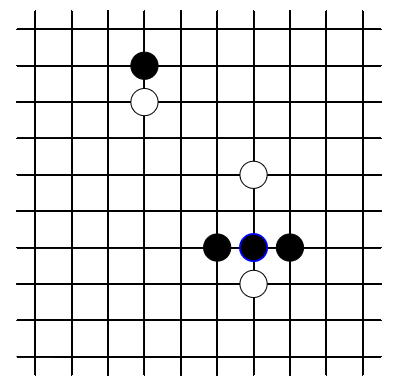
\includegraphics[scale=0.5]{fig2}
   \end{minipage} \hfill
   \begin{minipage}[c]{.46\linewidth}
       $\begin{pmatrix}
           0 & 1 & 2 & 1 & 2 & 1 & 1 & 0 & 0 & 0 \\
           1 & 1 & 2 & -1 & 2 & 1 & 1 & 1 & 0 & 1 \\
           1 & 1 & 2 & -1 & 2 & 1 & 1 & 0 & 1 & 0 \\
           0 & 1 & 1 & 1 & 1 & 1 & 1 & 1 & 1 & 1 \\
           1 & 1 & 1 & 1 & 1 & 1 & -1 & 1 & 1 & 1 \\
           1 & 0 & 0 & 1 & 2 & 2 & 1 & 2 & 1 & 0 \\
           0 & 1 & 1 & 1 & 4 & -1 & -1 & -1 & 4 & 1 \\
           0 & 0 & 0 & 1 & 2 & 2 & -1 & 2 & 2 & 1 \\
           0 & 0 & 1 & 1 & 1 & 1 & 1 & 1 & 1 & 1 \\
           0 & 0 & 1 & 1 & 1 & 1 & 1 & 1 & 1 & 1 \\
       \end{pmatrix}$
   \end{minipage}
\end{figure}

Cette matrice est mise à jour de la manière suivante : lorsque la fonction \verb+play+ du joueur est appelée, pour chaque nouveau coup \verb+(i, j)+, on met à jour la case concernée par le coup à \verb+-1+ (elle est en effet condamnée, on ne peut plus y jouer), ainsi que toutes les cases dont la valeur peut dépendre de \verb+(i, j)+. Ces cases forment une étoile autour de \verb+(i, j)+, comme le montre la figure \ref{fig:checkmove}.

Le principal intérêt de cette méthode est de permettre une estimation rapide de la valeur d'un coup et de la conserver pour plus tard durant la partie.

L'heuristique dépend de trois paramètres qui peuvent être modifiés durant la partie.
\begin{itemize}
    \item \verb+depth+ : la profondeur de l'arbre minimax à explorer
    \item \verb+nb_moves+ : le nombre maximum de coup à générer pour chaque joueur, le double de ce nombre constitue le nombre maximal de fils possible
    \item \verb+nb_layers+ : le nombre de valeurs de coups différentes à prendre, en commençant par les plus grandes.
\end{itemize}

Au tout début de la partie, il y a très peu de coups joués donc on n'est pas obligé de chercher très profond, en revanche on peut chercher plus large, car le nombre de possibilité est très grand. C'est pourquoi au fur et à mesure de l'avancement de la partie, on peut (doit) augmenter la profondeur de l'arbre et réduire un peu la largeur afin d'accélérer un peu le processus.

\subsubsection{Choix des Coups} \label{coups}

La matrice précédente sur la Figure \ref{fig1} permet d'avoir une estimation de la qualité d'un coup, il faut maintenant savoir quels coups choisir et combien de coups choisir. Pour cela les coups sont triés par catégorie (ceux de même valeur ensemble) puis on sélectionne avec deux limites :
\begin{itemize}
    \item on fixe le nombre maximal de valeurs différentes qui seront choisies
    \item on fixe un nombre maximal de coups qui peuvent être choisis
\end{itemize}

Les coups sont triés en utilisant un tableau à deux dimensions où chaque premier indice correspond à une valeur de coup, puis on utilise un curseur pour savoir où mettre un coup dans la ligne correspondante à sa valeur. Un tableau de curseurs est donc aussi nécessaire.

Ces limites sont variables selon l'avancement de la partie et ont été fixé à 3 pour le nombre de valeurs différentes et 6 pour le nombre de coups. Ainsi, si par exemple il y a 3 coups à 7, 5 à 4, 9 à 2 et 15 à 1, seront choisis les 3 coups à 7 et les 3 premiers coups de valeurs 4. Cette méthode permet de ne pas se focaliser trop uniquement sur les meilleurs coups et apportent des coups dont l'évaluation est moins bonne mais pour lesquels le futur pourrait être meilleur, l'heuristique n'étant qu'une approximation.

Cette opération est réalisée pour les deux opposants, afin d'empêcher l'adversaire de gagner s'il le faut. De ce fait, le nombre total maximal de fils pour un noeud est 12. Une fonction de concaténation de deux listes est donc implémentée, cette fonction vérifie au préalable linéairement si le coup de la seconde liste n'est pas déjà dans la première avant de l'ajouter.

\subsubsection{Évaluation du Plateau}
\label{evalplateau}

Les feuilles de l'arbre doivent donner une estimation de l'avantage du joueur pour l'avancement de la partie. On a choisi ici de réaliser la soustraction de la somme des éléments de chacune des deux matrices (opportunité et danger). Cela permet de donner la somme des longueurs de ligne déjà réalisées, moins celle de l'adversaire. Cette évaluation est ainsi très rapide car les matrices sont mises à jour sur les noeuds précédents.

Le principal problème de cette méthode provient du nombre de coups joués précédemment. En effet, comme les joueurs jouent l'un après l'autre, une fois sur deux, le premier joueur à un pion de plus posé sur le plateau. De ce fait le premier joueur a plus de lignes potentielles et donc cette évaluation est biaisée en sa faveur. Cela peut alors poser problème sur la profondeur de l'arbre explorée par le minimax.


\begin{itemize}
    \item Si cette profondeur est impaire et si le joueur est le premier à jouer, il obtiendra alors des évaluations biaisées en sa faveur, le rendant un peu trop optimiste.
    \item Si la profondeur est impaire et s'il est le second alors le biais disparaît
    \item Si la profondeur est paire et s'il est premier alors il n'y a pas de biais
    \item Si la profondeur est paire et s'il est second alors le biais sera en sa défaveur, rendant le joueur plus pessimiste.
\end{itemize}

Sachant qu'être pessimiste conduit à mieux se défendre alors qu'être optimiste conduit à attaquer trop librement (et donc de faire des erreurs), il vaut mieux avoir toujours une profondeur paire. Ce constat est vérifié par l'expérience, le joueur gagne plus souvent avec une profondeur paire.

Un second problème est qu'elle estime mal l'avantage du joueur si les pions sont très dispersés sur le plateau. En effet, cela créé des dizaines de lignes courtes potentielles dont la somme peut faire croire que l'adversaire à l'avantage. Ce phénomène explique pourquoi nos joueurs sont parfois un peu trop défensifs face à des joueurs aléatoires. Cet effet s'estompe un peu avec l'heuristique qui prend en compte les croisements car ils seront moins nombreux.

\subsubsection{Fonctionnement Negamax}

Le Negamax est une variante du minimax dans laquelle on considère que \verb+min(a,b) = -max(-a, -b)+. Cette écriture permet de raccourcir le code du minimax sans en changer le principe. Ce principe est le suivant : à partir d'un plateau, générer tous les coups intéressants, simuler ses coups, sélectionner le meilleur des coups et remonter sa valeur. \\

Deux systèmes permettent la gestion des coups. Celui des premiers joueurs était d'utiliser un type abstrait de données liste de coups qui permet d'ajouter des coups en fin de liste uniquement. Il interdit la suppression (mais on n'en a pas besoin) et permet aussi la concaténation de liste en évitant les doublons. Une seconde approche consiste à utiliser une pile. L'arbre des coups possibles est parcouru en profondeur, de ce fait on peut utiliser une pile pour stocker les coups que l'on considère au fur et à mesure. Cette pile est globale par rapport à la récursion du minimax afin d'éviter les réallocations. L'algorithme est récursif et les coups sont simulés en les ajoutant et les enlevant du plateau conservé par le joueur. On évite ainsi de faire des copies, opérations plus coûteuses.

Un problème qui se pose est le suivant : que faire lorsque le minimax remonte plusieurs coups qui ont la même valeur ? Nous avons ici considéré que prendre le premier coup de valeur maximale est la méthode la plus simple. En effet, il n'est pas nécessaire de surcharger le programme ici, et le meilleur moyen de résoudre le problème étant peut-être d'affiner l'heuristique afin que ce genre de cas se reproduise le moins souvent possible.

L'expérience montre cependant que ne pas prendre le premier change le déroulement de la partie ainsi que son issue. Les joueurs 4.4 et 4.3 n'ont pas les coups dans le même ordre et de ce fait font des choix différents.


\subsubsection{Élagage Alpha - Bêta}

\begin{figure}
    \centering
    \caption{Arbre de la figure \ref{arbre1} élagué}
    \label{arbre2}
    \begin{tikzpicture}[->,>=stealth',level/.style={sibling distance = 5cm/#1, level distance = 1.5cm}]
  \centering
\node  {5}
    child{ node  {5}
            child{ node  {5}
            	child{ node  {5} }
							child{ node  {-1}}
            }
            child{ node  {8}
							child{ node  {8}}
			}
    }
    child{ node  {4}
            child{ node  {4}
							child{ node  {4}}
							child{ node  {-9}}
            }
    }
;

\end{tikzpicture}
\end{figure}

Afin de gagner du temps de calcul, on cherche ici à éliminer les noeuds dont on est sûr que l'évaluation n'apportera rien à la valeur finale. Pour cela on fixe deux entier \verb+alpha+ et \verb+bêta+ qui vaudront respectivement le maximum et le minimum précédent. Ainsi par exemple, on sait que si l'on minimise et qu'on trouve une valeur plus grande que le minimum précédent, il n'est pas nécessaire de poursuivre sur cette branche car ce sera la valeur précédente qui sera retenue. Cette astuce provient du fait que l'on alterne maximisation et minimisation. \\
L'implémentation de cette solution est aisée, \verb+alpha+ et \verb+bêta+ sont passés en paramètre, à chaque coup analysé, on met à jour alpha comme maximum entre l'\verb+alpha+ précédent et la valeur du coup, et \verb+bêta+ comme le minimum. Si \verb+alpha+ passe au dessus de \verb+bêta+ c'est que ce coup est de moins bonne qualité qu'un coup précédent, son calcul n'apportera rien au résultat final, on arrête tout de suite de parcourir la branche.

\subsubsection{Multithreading}

Le parcours de l'arbre peut être fait en parallèle. Pour cela, on lance un thread pour chaque fils de la racine de l'arbre (l'état actuel réel du jeu). Étant donné que l'on ne connaît pas le nombre de fils de la racine à l'avance, il était plus facile de lancer tous les threads d'un coup sans se soucier du nombre de coeurs de la machine. Cela nous fait perdre l'amélioration de \verb+alpha+ \verb+bêta+ sur le premier niveau de l'arbre, mais le bénéfice de vitesse est plus grand. Cette opération nécessite cependant la copie de l'heuristique pour chaque thread. En effet, les simulations se passant en parallèle, chaque thread aura besoin d'un plateau de jeu sur lequel jouer et enlever les coups sans gêner les autres thread. Une structure de données est donc nécessaire pour faire le lien avec le thread. Celle-ci contient une copie de l'heuristique ainsi qu'un champ pour récupérer les résultats des simulations.

\begin{lstlisting}
    struct data{
        struct move_t mv;
        int step;
        struct heuristic * cp;
    };
\end{lstlisting}

La commande \verb+time+ de Linux nous donne le temps réel écoulé pendant l'exécution d'un programme, le temps total CPU (somme des temps passés dans chaque processeur) et le temps CPU passé en mode système. Appliqué à nos joueurs, on obtient le tableau figure \ref{tab2} sur un système 8 coeurs à 2.6 GHz. Ces valeurs nous permettent de dire que grâce au multithreading, on divise le temps nécessaire par 5 sur cette machine \footnote{La forge donne des timeout de plus de 40 secondes}. A noter que le joueur 4.1 n'est pas multithreadé et possède un arbre de recherche bien moins large ce qui explique sa rapidité.
\begin{figure}[h]
    \centering
    \caption{Temps sur les parties pour des joueurs multithreadés (4.4 et 4.3)}
    \label{tab2}
    \begin{tabular}{|c|c|c|c|c|}
    \hline
        Joueurs & Temps réel & Temps CPU user & temps CPU système & Nombre de tours de jeu\\
        \hline
         4.3 vs aléatoire & 4.2s & 27.9s & 0.02s & 13\\
        \hline
        4.1 vs 4.3 & 2.9s & 15.4s & 0.02s & 29 \\
        \hline
        4.4 vs 4.3 & 5.5s & 34s & 0.03s & 22\\
        \hline
    \end{tabular}
\end{figure}

Ce tableau montre bien le gain apporté par le calcul parallèle. Les parties sont jouées sur un plateau de taille $10\times 10$.

\subsection{Méthode de Monte Carlo}

\subsubsection{Principe Général}

La méthode de Monte Carlo est ici utile dans le contexte de l'arbre de recherche qu'est l'arbre des coups possibles. L'arbre réalisé par l'algorithme est en partie similaire à celui du minimax, chaque noeud est une configuration du jeu. Une feuille de l'arbre est soit un état final (partie terminée), soit une configuration du jeu à explorer. Chaque noeud de l'arbre contient deux valeurs : le nombre de simulations gagnantes et le nombre de simulations totales auxquelles le noeud à participer. \\

Une structure d'arbre est nécessaire ici pour se remémorer tous les états, cette structure n'était pas nécessaire pour le minimax qui était de nature récursive. La structure choisie est un type noeud ayant un tableau dynamique de successeurs de type noeud, ainsi qu'un pointeur vers le père du noeud. De cette manière on peut descendre et remonter l'arbre aisément. \\

\subsubsection{Algorithme}

L'algorithme repose sur la répétition des quatre phases suivantes :
\begin{itemize}
    \item la sélection : choisir une feuille de l'arbre non explorée
    \item l'expansion : ajouter à cette feuille tous les coups suivants possibles
    \item la simulation : simuler aléatoirement une partie à partir de chacun de ces nouveaux noeuds
    \item la mise à jour : mettre à jour les champs nombre de victoires - nombre de simulations pour chacun de ces noeuds, ainsi que pour l'ensemble de leurs ancêtres jusqu'à la racine.
\end{itemize}
Ce processus est répété des centaines de fois, on peut alors choisir l'un des fils de la racine comme prochain coup à jouer.

La méthode pour sélectionner une feuille est la suivante : on part de la racine, pour tout les fils, on choisit celui qui maximise la formule\footnote{Formule tirée de Wikipédia} :
\begin{equation}
    \frac{n}{N} + \sqrt{ 2 \times \log{\frac{N_{pere}}{N}}}
\end{equation}
où $n$ est le nombre de victoire du noeud, $N$ le nombre de simulations total du noeud et $N_{pere}$ le nombre de simulations total du père du noeud. On réitère ensuite sur ce nouveau jusqu'à atteindre une feuille. Cette solution permet de faire la part entre les noeuds qui apporte souvent de bons résultats (taux de victoire élevé) et ceux encore non explorés. \\

Les simulations consistent en des parties jouées de manière totalement aléatoire. C'est la répétition des simulations qui permet d'obtenir une approximation de la valeur d'un coup. Cette méthode a l'avantage de ne pas nécessiter de fonction d'évaluation de plateau. C'est là la force de cette algorithme, il est donc réutilisable pour tout type de jeu.


\section{Évaluation des Stratégies}

Quatre versions du joueur Minimax ont été implémentées. Cette section aborde leur spécification.

\subsection{Performance des Joueurs Minimax}

La figure \ref{tab3} nous donne les performances en termes de nombre de noeuds visités et temps nécessaire à leur visite par les quatre joueurs utilisant l'algorithme minimax. Ces tests ont été réalisé sur un plateau de taille $10 \times 10$.

Le joueur 4.1 dispose d'une heuristique très floue, de seulement 5 niveaux, ce qui fait qu'il peut calculer rapidement beaucoup de noeuds. L'inconvénient est que beaucoup d'entre eux ont des valeurs identiques, de ce fait il est plus difficile de contrôler la largeur de l'arbre. En effet, si on souhaite avoir des coups de valeurs maximales ainsi que quelques uns de moins bonne qualité, il risque d'y en avoir beaucoup (par exemple 2 de valeur 3 et 15 de valeur 2), sachant que l'opération est à réaliser pour les deux joueurs, il faut absolument contrôler la largeur. De ce fait il faut pouvoir décider quels noeuds choisir, alors qu'ils ont tous une valeur identique. C'est pourquoi il a été décidé que le joueur 4.1 ne considérerait que les coups de valeur maximal (amenant à une largeur petite), tandis que l'heuristique sera affinée pour les joueurs suivant.

Le joueur 4.2 dispose de la même heuristique que le joueur 4.1, la seule différence réside dans le parcours de l'arbre des coups possibles. Ce joueur ne se limite pas en profondeur mais en nombre de noeuds à visiter. La valeur par défaut donnée étant 10000 noeuds à visiter par appel à la fonction \verb+play+. Un accroissement de cette valeur n'a pas donné de bien meilleurs résultats, même à 100000 noeuds, il est incapable de battre le joueur 4.1 (match nul) et est bien plus lent.

Le joueur 4.3 est muni d'une heuristique très fine utilisant le croisement des lignes, celle-ci est décrite en section \ref{heur}. De plus, ce joueur choisit ses coups sur plusieurs valeurs différentes, méthode décrite en section \ref{coups}, lui permettant ainsi d'avoir le contrôle sur sa largeur. On obtient un nombre de noeuds visités par seconde inférieur aux premiers joueurs mais les coups sont d'une très meilleur qualité, le rendant victorieux très souvent. Il est cependant accéléré en utilisant le multithreading, ce qui permet selon les processeurs utilisés de se ramener à une vitesse similaire aux précédentes.

Le joueur 4.4 est identique au joueur 4.3 à ceci près qu'il utilise une pile afin de stocker les coups qu'il analyse au lieu de réallouer une liste à chaque noeud de l'arbre.


\begin{figure}[h]
    \centering
    \caption{Performance des Joueurs Minimax, arrondi aux milliers}
    \label{tab3}
    \begin{tabular}{|c|c|c|c|c|}
    \hline
        Joueurs & Nombre moyen de noeuds visités & Vitesse moyenne (sans multithread) & Maximum observé\\
        \hline
         4.1 & 5000 & 50000 noeuds/s & 45000 \\
        \hline
        4.2 & 10000 & 50000 noeuds/s & 10000 \\
        \hline
        4.3 & 12000 & 12000 noeuds/s & 90000 \\
        \hline
        4.4 & 12000 & 12000 noeuds/s & 70000\\
        \hline
    \end{tabular}
\end{figure}

\subsection{Performance du Joueur Monte Carlo}

Le joueur utilisant l'arbre de Monte Carlo s'est montré finalement peu compétent tout en étant assez lent. Il est capable de battre des joueurs aléatoires et les coups qu'il joue ne sont pas si mauvais. Le nombre de répétitions est fixé à 300 et du multithreading est utilisé pour tenter de l'accélérer un peu (les simulations des nouveaux coups ajoutés peuvent être réalisées en parallèle). Une autre amélioration est la conservation de l'arbre construit entre chaque tour de jeu. En effet, les coups qui furent finalement joués par lui et par l'adversaire étant déjà dans l'arbre, on déplace la racine en suivant ces coups, on repart ainsi d'un arbre pour lequel on a déjà quelques noeuds. Ce joueur aurait pu être encore amélioré en l'aidant à choisir ses coups (plutôt qu'en lui faisant tout tester).

\subsection{Évaluation de l'Heuristique}
\label{evalheur}

On cherche ici à valider notre heuristique. Pour cela, on va vérifier si la valeur renvoyée par l'heuristique est bien corrélée avec sa probabilité de victoire. Pour chaque valeur, il faut dénombrer un nombre significatif de parties et compter le nombre de victoires pour le joueur pour lequel l'évaluation heuristique était destinée. Cependant, on ne peut pas calculer toutes les parties possibles, il y a en a beaucoup trop (de l'ordre de $2^{N\times N}$ avec $N$ la taille du plateau). On se limite donc à des parties effectuées sur un plateau de taille $7 \times 7$, sur lequel aura été posé au préalable 30 pions. En retirant le nombre de pions posés, il reste $2^{19}$ parties possibles pour chaque plateau, on prend 10 plateaux différents pour chaque valeur d'heuristique et on réalise 500 000 parties aléatoires sur chaque, soit un total de 5 millions de parties.


\begin{figure}[h]
    \centering
    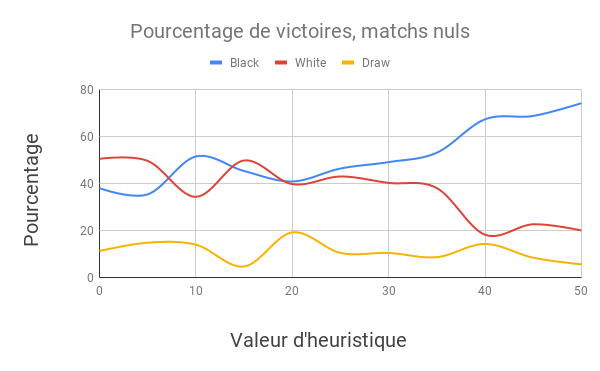
\includegraphics[scale=0.8]{Pourcentage_de_victoires_matchs_nuls.png}
    \caption{Pourcentage de parties gagnées pour les Noirs et les Blancs en fonction de la valeur prédite de l'avantage des noirs}
    \label{fig:stats1}
\end{figure}

La figure \ref{fig:stats1} montre les courbes obtenues selon les spécifications données plus haut. On constate que le pourcentage de victoire semble croître avec la valeur d'heuristique comme attendu. Cependant les résultats sont incertains pour des valeurs petites (inférieure à 20). Ces résultats sont de plus à prendre avec des pincettes, les plateaux étant générés aléatoirement, ils doivent avoir un fort taux de dispersion ce qui fausse un peu l'heuristique comme expliquée en section \ref{evalplateau}. C'est pourquoi des tests sur des plateaux issues de parties réels ont été réalisé. Les parties furent réalisées sur des plateaux de taille $10\times 10$ et on a réalisé 100 millions de parties. On constate que la corrélation semble toujours être bonne.


\begin{figure}[h]
    \centering
    \caption{Tests d'heuristique sur des parties plus "plausible"}
    \label{tab4}
    \begin{tabular}{|c|c|c|c|c|}
    \hline
        Valeur d'heuristique & Victoire des noirs & Victoire des blancs & Match nuls\\
        \hline
        -8 & 37 290 189 & 62 468 415 & 241 396 \\
        \hline
        15 & 59 979 045 & 39 972 117 & 48 838 \\
        \hline
        24 & 65 469 322 & 34 509 156 & 21 522 \\
        \hline
        36 & 79 160 262 & 20 831 901 & 7 837\\
        \hline
        44 & 73 205 647 & 26 777 715 & 16 638\\
        \hline
    \end{tabular}
\end{figure}


\section{Évaluation des Ouvertures}

Une évaluation des différentes ouvertures nous est proposé sur la page Wikipédia et il nous est demandé de tester si nous obtenons des résultats similaires à ceux présentés sur la page. Il convient cependant, d'analyser ce qui est indiqué. Il est écrit par exemple pour certains openings : victoire certaine du joueur BLACK. Néanmoins il ne faut pas le comprendre comme : le joueur BLACK peut jouer les coups qu'il veut dans tous les cas il gagnera. En effet il est très simple au Gomoku de laisser gagner son adversaire. Il faut plutôt l'entendre comme : si la stratégie jouée est optimale, avec un tel début de partie sa victoire est assurée. Ainsi qu'est ce que la façon optimale de jouer ? On ne connaît pas à notre échelle cette manière de jouer, nous pouvons en effet tester toutes les parties qui pourraient se dérouler mais on ne peut pas choisir qu'elles seront, parmi ces parties, les parties qui correspondent aux parties optimales dans la manière de jouer. Ainsi si nous voulions le faire, il faudrait:
\begin{enumerate}
    \item Créer un opening
    \item réaliser un grand nombre de match différents entre deux joueurs jouant de manière parfaite
    \item noter les résultats
\end{enumerate}


\section{Conclusion}
\label{sct:ccl}
Durant ce projet nous avons essayé de rester le plus générique possible. L'implémentation de différents types abstraits de données nous a semblé être la bonne solution pour l'être, notamment dans l'implémentation du serveur. Nous avons aussi essayé de nous inscrire dans une démarche scientifique durant l'analyse de nos fonctions d'évaluations. Grâce à plusieurs dialogues nous avons pu vous présenter nos tests sur la fonction heuristique dans notre partie \ref{evalheur}, permettant de montrer qu'elle renvoie des valeurs assez cohérentes et proches de la probabilité de gagner à partir de 30 tours sur un plateau 7*7 par exemple.

% après faut parler d'améliorations, mais je les ai déjà évoqué dans mes parties

\end{document}
